% Slides accompanying "Learn RISC-V CPU Implementation and BSV" book
% Copyright (c) 2024 Rishiyur S. Nikhil, All Rights Reserved

% -*- mode: fundamental -*-

% Slides accompanying "Learn RISC-V CPU Implementation and BSV" book
% Copyright (c) 2024 Rishiyur S. Nikhil, All Rights Reserved

% This is a preamble shared by all the slide decks

\documentclass[10pt, aspectratio=169]{beamer}

% \documentclass[17pt]{beamer}

% Avail. font sizes: 8pt, 9pt, 10pt, 11pt, 12pt, 14pt, 17pt, 20pt.
% Default font size is 11pt (= 22pt in full screen mode).

\usepackage{verbatim}
\usepackage{fancyvrb}
\usepackage{listings}

\usepackage{array}

% ================================================================
% Themes

\usetheme{Madrid}          % Line at bottom: Author (affiliation), OptTitle, Conf, page 

% \usetheme{Copenhagen}    % Same as Madrid except bottom line: Author, OptTitle

% \usetheme{Berkeley}    % Takes up 1-inch border on left and top

% ----------------
% colorthemes
% (default), beaver, beetle, seahorse, wolverine

\usecolortheme{seahorse}

% ================================================================
% Customization: show table of contents before each section
% Use \AtBeginSubsection    to show before each subsection

% \AtBeginSection[]
% {
%   \begin{frame}
%     \frametitle{Table of Contents}
%     \tableofcontents[currentsection]
%   \end{frame}
% }

% ================================================================

% ----------------
% The bsc compiler and BSV language
\newcommand{\bsc}{\emph{bsc}}
\newcommand{\BSV}{\bf{BSV}}
% ----------------
% ITALICISE WORDS
\newcommand{\ie}{\emph{i.e.,}}
\newcommand{\eg}{\emph{e.g.,}}
\newcommand{\Eg}{\emph{E.g.,}}
\newcommand{\etc}{\emph{etc.}}
\newcommand{\via}{\emph{via}}
\newcommand{\vs}{\emph{vs.}}

% ----------------
% EMPTY BOXES OF VARIOUS WIDTHS, FOR INDENTATION (N 'em' spaces)

\newcommand{\hm}{\hspace*{1em}}
\newcommand{\hmm}{\hspace*{2em}}
\newcommand{\hmmm}{\hspace*{3em}}
\newcommand{\hmmmm}{\hspace*{4em}}

% ----------------
% Convenient widths (less than text width by N 'em' spaces)

\newlength{\hlessmm}
\setlength{\hlessmm}{\textwidth}
\addtolength{\hlessmm}{-2em}

\newlength{\hlessmmm}
\setlength{\hlessmmm}{\textwidth}
\addtolength{\hlessmmm}{-3em}

\newlength{\hlessmmmm}
\setlength{\hlessmmmm}{\textwidth}
\addtolength{\hlessmmmm}{-4em}

% ----------------
% EMPTY LINES of various heights  (N 'ex' heights)

\newcommand{\vx}{\vspace*{1ex}}
\newcommand{\vxx}{\vspace*{2ex}}
\newcommand{\vxxx}{\cspace*{3ex}}
\newcommand{\vxxxx}{\vspace*{4ex}}

% ----------------
% Inputting verbatim code fragments, with various font sizes

\newcommand{\SHOWCODE}[1]{{\footnotesize\input{#1}}}

\newcommand{\SHOWCODESCRIPT}[1]{{\scriptsize\input{#1}}}

\newcommand{\SHOWCODETINY}[1]{{\tiny\input{#1}}}

% ----------------
% To allow redefinition of "pause" during development vs. deployment
% Argument is vertical space command

% Choose with or without pauses
% \newcommand{\PAUSE}[1]{#1\pause}
\newcommand{\PAUSE}[1]{#1}

% ----------------
% Emojis

\graphicspath{ {./../Figures/} }

\newcommand{\EmojiExercise}{\begin{minipage}[c]{5em}
  \includegraphics[width=3em]
    {person-lifting-weights-emoji-clipart-md-3307277008.png}
\end{minipage}}

% ================================================================
% Title page

\title[Learn CPU design \& {\BSV}]{Learn RISC-V CPU Implementation and {\BSV}}

\subtitle{({\BSV}: a High-Level Hardware Design Language)}

\author[{\copyright} R.S.Nikhil]{Rishiyur S.~Nikhil}
% \institute{Bluespec, Inc.}

% Date is set differently in each slide deck

% \logo{\includegraphics[height=0.6cm]{../Figures/Bluespec_Logo_2022-10}}

% End of preamble
% ****************************************************************


\date{L18: RISC-V: Optimizing Drum and Fife}

% ****************************************************************

\begin{document}

% ================================================================

\begin{frame}
\titlepage

\begin{center}
 \includegraphics[height=1cm]{Bluespec_Logo_2022-10}
\end{center}

\end{frame}

% ================================================================

\section{Reminders}

% -*- mode: fundamental -*-

% ================================================================

\begin{frame}[fragile]
\frametitle{Reminders}

\footnotesize

Please git clone: \url{https://github.com/rsnikhil/Learn_Bluespec_and_RISCV_Design} \\
(git pull for latest version).  Repsitory structure:

\vspace{1ex}

\begin{minipage}{0.5\textwidth}\scriptsize
\begin{Verbatim}[frame=single, numbers=left]
    ./Book_BLang_RISCV.pdf
      Slides/
          Slides_01_Intro.pdf
          Slides_02_ISA.pdf
          ...
      Exercises/
          Ex-03-A-Hello-World/
          Ex-03-B-Top-and-DUT/
          ...
      Code/
          src_Top/
          src_Drum/
          src_Fife/
          src_Common/
          ...
      Doc/Installing_bsc_Verilator_etc.{adoc,html}
\end{Verbatim}
\end{minipage}
\hm
\begin{minipage}{0.45\textwidth}
\begin{itemize}

 \item Slides and Exercise are numbered in sync with book Chapter numbers.

 \item For Exercises, please see Appendix E of the book.  Some (not
       all) exercises have associated code in the {\tt Exercises/}
       directory.

\end{itemize}
\end{minipage}

\vspace{2ex}

To compile and run the code for exercises, Drum and Fife, please make sure you have installed:

\begin{itemize}

 \item \emph{bsc} compiler (see \url{https://github.com/B-Lang-org/bsc})

 \item Verilator compiler (see \url{https://www.verilator.org/})
\end{itemize}

\footnotesize

\end{frame}

% ================================================================

\begin{frame}
\frametitle{Chapter Roadmap}

\footnotesize

\begin{center}
\frame{\includegraphics[height=0.825\textheight]{Fig_Chapter_Roadmap}}
\end{center}

\end{frame}

% ================================================================


% ================================================================

\begin{frame}
\frametitle{Table of Contents}

\tableofcontents

\end{frame}

% ****************************************************************

\section{General Comments}

\begin{frame}

\begin{center}
  {\LARGE General Comments}
\end{center}

\end{frame}

% ================================================================

\begin{frame}[fragile]
\frametitle{What are we optimizing?}

\footnotesize

Three physical dimensions for optimization:

\vxx

\begin{itemize}

  \item Time (performance): how fast (wall-clock time) does the CPU execute an application?

  \vx

  \item Space (area/resources): how much silicon area is taken up by the design
      (measured in gates, LUTs
      (lookup tables), BRAMs (block SRAMs), memories, DSPs, wiring
      congestion, {\etc})?

  \vx

  \item Energy: how much energy is consumed to execute an application?

\end{itemize}

\vxx

These dimensions are not independent--an improvement in one may
require a worsening in another (tradeoff).

\vx

Ultimately, a competitive product specification for a particular target
market will define the acceptable boundaries for each dimension.

\vx

There is no easy way to estimate energy consumption other than actual
measurement---run an application and measure the energe consumption.
Optimizing energy consumption involves techniques such as lowering
clock speeds and/or supply voltages dynamically during less critical
periods.

\vx

\begin{center}\large
\emph{Our focus here is on space/time tradeoffs.}
\end{center}

\end{frame}

% ================================================================

\begin{frame}[fragile]
\frametitle{CPU Performance}

\footnotesize

The time to execute an application is a product of multiple terms:

\begin{tabbing}
\hmmmm
\= {\tt <}exec time{\tt>}
\= $=$                   
\= {\tt <}total number of instrs{\tt >}
\= \hm $\times$ \hm
\= $1/${\tt <}clock-speed{\tt >}
\= \hm $\times$ \hm
\= CPI
\end{tabbing}

the units being:

\begin{tabbing}
\hmmmm
\= {\tt <}exec time{\tt>}
\= $=$                   
\= {\tt <}total number of instrs{\tt >}
\= \hm $\times$ \hm
\= $1/${\tt <}clock speed{\tt >}
\= \hm $\times$ \hm
\= CPI
\kill
\> seconds
\> $=$
\> instructions
\> \hm $\times$ \hm
\> seconds/cycle
\> \hm $\times$ \hm
\> cycles/instruction
\end{tabbing}

{\scriptsize ``cycles/instruction'' may vary depending on the type of
instruction ({\eg} integer {\vs} floating point), and what precedes
and follows an instruction (stalling due to register hazards, cache
misses on fetch or DMem op, ...), so this should be considered to be
an average.

\vx

``clock speed'' may vary during application execution, in some CPU
implementations; this should also be considered to be an average.}

\vx

\emph{NOTE}: \hm
\fbox{
\begin{minipage}{0.85\textwidth}

A design with a slower clock speed can have faster performance than a
design with a higher clock speed if it can perform the computation
with fewer instructions and/or with fewer cycles/instruction.

\vx

\scriptsize
In the early 1990s Digital Equipment Corporation's first Alpha
microprocessors had \emph{much} higher clock speeds than the
competition, but were often slower on benchmark applications because
of the other factors.

\end{minipage}}

\PAUSE{\vxx}

To improve performance we can try to improve each of the product terms:
\begin{itemize}

  \item Reduce number of instructions with different ISA ({\eg} RV32IM
      {\vs} RV32I; ARM {\vs} x86 {\vs} RISC-V)

  \item Reduce number of instructions with better coding) ({\eg} mergesort {\vs} bubblesort)

  \item Reduce number of instructions with better compiler

  \item Increase the clock speed

  \item Use fewer cycles to execute each instruction
\end{itemize}

\end{frame}

% ================================================================

\begin{frame}[fragile]
\frametitle{Area {\vs} Clock-speed tradeoffs}

\footnotesize

Increasing clock speed:
\begin{itemize}

  \item means each combinational path from one register's output to
      the next register's input can accommodate fewer gates, thereby
      doing less computation work.

  \item might require more stages in a pipeline, thereby increasing
      area due to inter-stage buffers and more inter-stage control
      circuitry (hand-shaking logic).

\end{itemize}

\PAUSE{\vxx}

\emph{Sharing} a hardware component ({\eg} sharing an adder for the
ADD instruction, for Load/Store effective address calculation, for
BRANCH/JUMP address calculation, {\etc}):

\begin{itemize}
    \item Sharing a component can save area ... but ...

    \item requires a multiplexer on the input for the different input sources, and

    \item requires longer wiring to and from the component for its multiple uses, and

    \item requires control logic and possibly stalling logic to
        schedule the use of the component by its various users, ...

   \item all of which can result in higher area and longer delays (slower clock speed).
\end{itemize}

\end{frame}

% ================================================================

\begin{frame}[fragile]
\frametitle{Transformations to ``balance'' a pipeline}

\footnotesize

The \emph{critical} path is the longest-delay combinational path in
the entire design.  The clock speed has to be slow enough to
accommodate this delay.

\vxx

\begin{itemize}

  \item Two adjacent pipeline stages whose combined delay is less than
      the critical path (in some other stage) can be \emph{fused} into
      a single stage without changing the clock speed.  This reduces
      the number of stages needed for any instruction.

  \item A stage with a long critical path can be \emph{split} into two
      stages to permit a higher clock speed.

      After the split, the critical path may remain with this stage,
      or may now be due to some other stage.

  \item Combinational logic in a stage with a long critical path may
      be \emph{moved} into the adjacent upstream or downstream stage.
      This will shorten the critical path of this stage while
      increasing the critical path of the adjacent stage.

      It may result in more or less inter-stage buffer space to hold
      the inter-stage value.

\end{itemize}

\vxx

Such transformations may be iterated to \emph{balance} the pipeline,
{\ie} have roughly equal delays in each stage.

\end{frame}

% ================================================================

\begin{frame}[fragile]
\frametitle{Pipeline traces for pipeline performance analysis}

\footnotesize

A \emph{pipeline trace} is a trace output from the CPU that is much
more detailed than an instruction trace (discussed in earlier chapters
on functional verification).

On each clock, the CPU outputs the state of each pipeline stage:

\begin{itemize}

  \item Which instruction (if any) is currently in that stage, along
      with additional information carried along with the instruction.

  \item The stage state: stalled due to empty input; stalled due to
      full output; stalled due to scoreboard; ...
\end{itemize}

Pipeline traces can be analyzed:

\begin{itemize}

  \item Manually: study the trace to detect issues

  \item Programmatically: an analysis program processes the trace looking for certain issues

  \item Visually (see next slide)

\end{itemize}

\end{frame}

% ================================================================

\begin{frame}[fragile]
\frametitle{Visualization of pipeline traces}

\footnotesize

A Pipeline trace can be visualized as in the following example:

\includegraphics[width=\textwidth]{Fig_PipeViz_Fife}

\begin{itemize}
  \item The y-axis (going downwards is ``inum'', the instruction number (serial number)
  \item The x-axis is time (each column is a clock tick).

  \item Each horizontal row represents one instruction traversing the
        pipeline, showing each stage (F=Fetch, D=Decode, EX.I=Execute
        Integer, RET.D=Retire DMem, RW=Register Write, ...).

\end{itemize}

Such a visualization dramatically highlights stalls (wasted cycles).

Once we see a stall, we can analyze that part of the pipeline trace in
more detail to identify the reason for the stall and propose an
improvement.  The improvement may merely be improved compilation
({\eg} rearrange instructions to reduce the likelihood of scoreboard
conflicts), or it could be an adjustment to the hardware design.

\end{frame}

% ****************************************************************

\section{Optimizing Drum/Fife}

\begin{frame}

\begin{center}
  {\LARGE Optimizing Drum and Fife}
\end{center}

\end{frame}

% ================================================================

\begin{frame}[fragile]
\frametitle{Fusing/splitting stages: Decode and Register-Read-and-Dispatch}

\footnotesize

\begin{center}
\includegraphics[width=0.9\textwidth]{Fig_RISCV_Fuse_Decode_RR}
\end{center}

\begin{itemize}\scriptsize

  \item The left-hand side depicts two stages. In Drum, a {\tt
      Decode\_to\_RR} struct is communicated from function {\tt
      fn\_Decode} to {\tt fn\_Dispatch} {\via} a register.  In Fife,
      it is communicated {\via} a FIFO.

  \item The right-hand size depicts a single \emph{fused} stage.  The
      value is communicated directly, by composing the functions
      directly (in hardware: just wires).

      \vx

      The inputs and outputs of the fused stage are exactly the same
      the inputs and outputs of the original two stages.

\end{itemize}

{\scriptsize \emph{Splitting} a stage into two is the exact inverse of fusing.}
\hfill
{\scriptsize Please see book Chapter 18 for {\BSV} code excerpts for fusing.}

\end{frame}

% ================================================================

\begin{frame}[fragile]
\frametitle{Fusing some Retire actions}

\footnotesize

In both Drum and Fife, exception handling is done in one place, by
itself.

\vx

In Drum, it is the last, separate action in the FSM,
\verb|a_exception|, in module \verb|mkCPU| in \verb|src_Drum/CPU.bsv|.

\vx

In Fife, it is in rule \verb|rl_exception| in module module
\verb|mkRetire| in \verb|src_Fife/S5_Retire.bsv|.

\PAUSE{\vxxxx}

In both cases, the exception is actually detected in earlier rules,
which save values in three registers \verb|rg_epc|, \verb|rg_cause|
and \verb|rg_tval| which are then used by the exception handling
action.

\vx

The exception-handling action can be fused directly into the earlier
actions where the exception was detected, and the three registers can
be eliminated.

\PAUSE{\vxxxx}

{\scriptsize This transformation may be less important because
exceptions should be rare, and therefore saving these few ticks may
not affect application performance very much.}

\end{frame}

% ================================================================

\begin{frame}[fragile]
\frametitle{Fife: saving FIFO resources}

\footnotesize

Section 16.3 with Figure 16.2 and Section 17.5.3 with Figure 17.7
describe how to connect Fife stages in a modular way, using a pair of
FIFOs---a BypassFIFO in one stage (module) and a PipelineFIFO in the
other, connected using \verb|mkConnection| in the parent CPU module.

\vx

Logically this is a 1-element FIFO, but we use these two FIFOs to
isolate the stages (separate rule scheduling, no combinational paths
through the FIFO).

\PAUSE{\vxx}

We could replace some FIFO pairs by a single FIFO, halving the
register count for that connection.  We lose isolation between stages
and introduce combinational paths, but this may be harmless in
selective cases.

\PAUSE{\vxxxx}

Whether we use a PipelineFIFO or a BypassFIFO for this purpose depends
on where it is used, because of the scheduling constraint.  Usually we
will need a PipelineFIFO in a forward path and a BypassFIFO in a
reverse path because, for pipeline behavior we need to schedule a
downstream rule before an upstream rule.

\end{frame}

% ****************************************************************

\section{Reducing misprediction penalty}

\begin{frame}

\begin{center}
  {\LARGE Fife: Reducing misprediction penalty}
\end{center}

\end{frame}

% ================================================================

\begin{frame}[fragile]
\frametitle{Fife: reducing misprediction penalty (1/3)}

\footnotesize

In Fife, the Fetch unit continually predicts the next PC so that it
can continue fetching and feeding the pipeline.  When it predicts
incorrectly, this is detected in Retire, which redirects Fetch to the
correct PC. In the meanwhile, Fetch has already fetched and fed a
number of instructions into the pipeline, which must now all be
discarded.  The cycles spent on discarding these mispredicted
instructions is called the \emph{misprediction penalty}.

\PAUSE{\vxxxx}
\vxxxx

% ----------------------------------------------------------------
\hdivider

{\bf Optimization: Use CRegs in Fetch for PC and epoch}

\vxx

In Fetch, the PC and epoch are ordinary registers.  The redirection
action writes these registers, and the fetch action reads them, which
can only happen on the next clock.

\vxx

\emph{Optimization:} By using CRegs for the PC and epoch, the
redirection-writes and the fetch-reads can be done in the same clock,
saving a tick.

\end{frame}

% ================================================================

\begin{frame}[fragile]
\frametitle{Fife: reducing misprediction penalty (2/3)}

\footnotesize

% ----------------------------------------------------------------
\hdivider

{\bf Optimization: Eliminate FIFO on backward redirect path}

\vx

The redirection message from Retire to Fetch passes through a FIFO.

\vxx

\emph{Optimization:} Eliminate this FIFO; let the Retire stage
directly write into the PC and epoch registers in Fetch, saving a
clock tick.

\vx

{\emph{Caveat:}} less isolation between Retire and Fetch (longer
combination paths, more rule-scheduling constraints).

\PAUSE{\vxxxx}

% ----------------------------------------------------------------
\hdivider

{\bf Quicker reaction to redirection by Decode and Register-Read and Dispatch}

\vx

A mispredicted instruction may stall on the scoreboard, spend many
cycles in a long pipeline (memory, multiply/divide, floating-point),
and reserve various resources (Rd register, slot in DMem
store-buffer).

\vxx

{\emph{Optimization:}} When Retire redirects Fetch, also send the new
epoch to Decode and Register-Read-and-Dispatch.  They can immediately
start discarding wrong-epoch instructions and/or convert them into
no-ops, so they no longer reserve any resources or extra cycles.

\end{frame}

% ================================================================

\begin{frame}[fragile]
\frametitle{Fife: reducing misprediction penalty (3/3)}

\footnotesize

{\bf Optimization: More accurate PC prediction}

\vx

A PC-predictor is a function from PC to predicted-next-PC.  Currently
this function is very simple: just add 4 (predict PC+4).

\vx

This is not bad, but it mispredicts on BRANCH instructions where the
branch is taken and on JAL and JALR instructions.  It also fails on
traps (jump to PC in CSR {\tt mtvec}).

\vx

Improving the accuracy of PC-prediction is a vast topic: there are
many, many papers on this topic, spanning many decades, in premier
computer architecture conferences.

\PAUSE{\vx}

\hdivider

{\emph{Optimization:}} ``Branch Target Buffers'' (BTBs) are
associative tables, associating the PC of a BRANCH or jump instruction
with the target PC it branched/jumped to.  This information is updated
with accurate information from redirection messages.  The PC predictor
consults this table and, if it finds a matching entry for the current
PC, uses this value instead of PC+4 for the predicted PC.

\PAUSE{\vx}

\hdivider

{\emph{Optimization:}} A ``Return Address Stack'' is a small ``shadow
stack'' that mimics the saving and restoring of PCs on the real
program stack on function calls and returns.

\vx

A JAL/JALR is likely a function call if it saves the current PC in the
{\tt ra} register.  A JALR is likely a function return if it takes its
target PC from the {\tt ra} register.  When these are recognized, they
can push/pop PCs in the Return Address Stack, and these can be used
for PC prediction.

\end{frame}

% ****************************************************************

\section{Reducing register-hazard penalty}

\begin{frame}

\begin{center}
  {\LARGE Fife: Reducing register-hazard penalty}
\end{center}

\end{frame}

% ================================================================

\begin{frame}[fragile]
\frametitle{Fife: Reducing register-hazard penalty (1/3)}

\footnotesize

The \emph{register-hazard penalty} is the number of cycles an
instruction I2 may stall (idle wait) in the Register-Read stage
because one or more of its input or output registers are
``busy''---there is an earlier instruction I1 ahead of it in the
pipeline that will be writing to one of those registers.  This
``stall'' situation is detected and managed using the scoreboard.

\PAUSE{\vxxxx}

\hdivider

{\bf Optimization: Saving a tick from register-update to dispatch}

\vx

In stage {\tt S3\_RR\_RW}
\begin{itemize}

  \item[(A)] Rule {\tt rl\_RR\_Dispatch} reads and writes {\tt
      rg\_scoreboard} to manage register hazards, and reads one or two
      GPRs (in the {\tt mkGPRs} module).

  \item[(B)] Rule {\tt rl\_RW\_from\_Retire} reads and writes {\tt
      rg\_scoreboard} and writes zero or one GPRs (in the {\tt mkGPRs}
      module).

\end{itemize}

\vxx

Rule scheduling into clocks will therefore dictate that rule (A)
cannot see the effects of rule (B) until at least one clock later.

\vxx

{\emph{Optimization:}} Use CRegs for both {\tt rg\_scoreboard} and for
GPRs.  This will allow rule (A) to see the results of rule (B) in the
same clock, saving a tick.

\PAUSE{\vxx}

{\scriptsize\emph{Note:} {\tt mkGPRs} only needs a single {\tt
Bit\#(XLEN)} CReg at the interface; the actual GPRs can remain an
ordinary {\tt RegFile}.  See book Section 18.3.7.1 for how to do
this.}

\end{frame}

% ================================================================

\begin{frame}[fragile]
\frametitle{Fife: Reducing register-hazard penalty (2/3)}

\footnotesize

{\bf Optimization: Eliminate FIFO on backward register-update path}

\vx

The register-update message from Retire to Register-Read-and-Dispatch passes through a FIFO.

\vxx

\emph{Optimization:} Eliminate this FIFO; let the Retire stage
directly write into the GPRs and scoreboard in
Register-Read-and-Dispatch, saving a clock tick.

\vx

{\emph{Caveat:}} less isolation between Retire and
Register-Read-and-Dispatch (longer combination paths, more
rule-scheduling constraints).

\end{frame}

% ================================================================

\begin{frame}[fragile]
\frametitle{Fife: Reducing register-hazard penalty (3/3)}

\footnotesize

{\bf Optimization: Avoiding the stall on Rd}

\vx

Currently, an instruction I2 stalls in Register-Read-and-Dispatch if
it has the same Rd as some instruction I1 ahead of it in the pipeline,
because that register will have been reserved in the scoreboard.

\vxx

{\emph{Optimization:}} Generalize the scoreboard from a single bit
(``free''/``busy'') to a small up-down counter (say 2 or 3 bits).  In
Register-Read-and-Dispatch, when dispatching an instruction,

\begin{itemize}

  \item Stall it if the counter for its Rs1 or Rs2 is non-zero.

  \item If the counter for its Rd is not ``saturated'' (at its maximum
      value), increment the counter and allow the instruction to
      proceed (do not stall).

\end{itemize}

In Register-Read-and-Dispatch, when we receive a register update
message from Retire, decrement the counter for Rd.

\vx

Use a CReg for each register's scoreboard up-down counter, as
described in Chapter~17, to allow the register-update and dispatch in
the same cycle.

\end{frame}

% ****************************************************************

\section{Final Comments}

\begin{frame}[fragile]
\frametitle{Final comments on Optimization}

\footnotesize

This chapter has limited itself to optimizations that do not
fundamentally change the microarchitecture of Fife and Drum, and has
avoided discussing more radical changes (to superscalar, out-of-order,
{\etc}).  The latter are briefly discussed in Chapter~20.  As such,
the optimizations discussed here are relatively local and
non-disruptive.

\vxx

The major ideas are:

\begin{itemize}

 \item Fusion and splitting of stages and actions

 \item Using leaner FIFOs

 \item Improving accuracy of PC-prediction, and reacting more quickly to misprediction

 \item Sharing circuits (less area, but more MUXes and control logic) and un-sharing

 \item Using CRegs to save clock ticks

 \item Eliminating the stall on Rd

\end{itemize}

\end{frame}

% ****************************************************************

% -*- mode: fundamental -*-

% Slides accompanying "Learn RISC-V CPU Implementation and BSV" book
% Copyright (c) 2024 Rishiyur S. Nikhil, All Rights Reserved

% This is a postamble shared by all the slide decks

% ================================================================

\begin{frame}

\begin{center}
  {\LARGE End}
\end{center}

\end{frame}

% ================================================================


% ****************************************************************

\end{document}

% ****************************************************************
